\newpage
\section{Naive Bayes}
\label{sec:naive-bayes}

This section evaluates Naive Bayes classifiers as the first explicitly generative model family in the project. Logistic regression directly models the posterior probability \(P(Y=1\mid X=x)\), and k-nearest neighbours predicts from local similarity in the transformed feature space. Naive Bayes instead models the class prior and the feature distribution within each class, then applies Bayes' rule to obtain posterior class probabilities.

The same training-only validation discipline is used as in the previous modelling sections. The held-out test set remains unused. All reported results are based on stratified cross-validation inside the training set, using out-of-fold predictions.

\subsection{Bayes classifier}

For binary classification, the ideal classifier predicts the class with the largest true posterior probability:
\[
h^\star(x)
=
\arg\max_{y\in\{0,1\}}
P(Y=y\mid X=x).
\]
For churn classification, where \(Y=1\) denotes churn and \(Y=0\) denotes no churn, this can be written as
\[
h^\star(x)
=
\mathbb{1}
\left\{
P(Y=1\mid X=x)\geq 0.5
\right\}.
\]
This rule is called the Bayes classifier. It is ideal because it uses the true conditional probability of the class given the features. In practice, this posterior probability is unknown and must be estimated from data.

Under 0-1 loss, the risk of a classifier \(h\) is
\[
R(h)
=
P(h(X)\neq Y)
=
\mathbb{E}
\left[
\mathbb{1}\{h(X)\neq Y\}
\right].
\]
The Bayes classifier minimizes this risk over all possible classifiers:
\[
h^\star
=
\arg\min_h R(h).
\]
The corresponding minimum possible error rate is the Bayes risk,
\[
R^\star
=
R(h^\star).
\]
For binary classification, the Bayes risk can be written as
\[
R^\star
=
\mathbb{E}_X
\left[
\min
\{
P(Y=0\mid X),
P(Y=1\mid X)
\}
\right].
\]
This expression shows that classification error can be irreducible. If churners and non-churners overlap for the same observed feature values, then even the ideal classifier must sometimes be wrong.

\subsection{Bayes decision rule and unequal costs}

The threshold \(0.5\) is optimal only when false positives and false negatives have equal cost. In churn prediction, this is not necessarily realistic. A false positive may cause unnecessary retention effort, while a false negative may mean missing a customer who will leave.

Let \(C_{\mathrm{FP}}\) denote the cost of a false positive and \(C_{\mathrm{FN}}\) the cost of a false negative. A cost-sensitive Bayes decision rule predicts churn when
\[
C_{\mathrm{FP}}P(Y=0\mid X=x)
\leq
C_{\mathrm{FN}}P(Y=1\mid X=x).
\]
Equivalently, predict churn when
\[
P(Y=1\mid X=x)
\geq
\frac{C_{\mathrm{FP}}}{C_{\mathrm{FP}}+C_{\mathrm{FN}}}.
\]
If missing a churner is more costly than unnecessarily contacting a non-churner, then \(C_{\mathrm{FN}}>C_{\mathrm{FP}}\), and the optimal threshold is below \(0.5\). This provides the theoretical reason why the project studies threshold tradeoffs for probabilistic classifiers.

\subsection{Bayes' rule and generative classification}

Bayes' rule gives
\[
P(Y=y\mid X=x)
=
\frac{
P(X=x\mid Y=y)P(Y=y)
}{
P(X=x)
}.
\]
For classification, the denominator \(P(X=x)\) is the same for every class. Therefore, the predicted class can be obtained by comparing the unnormalized posterior scores:
\[
\widehat{y}
=
\arg\max_{y\in\{0,1\}}
P(X=x\mid Y=y)P(Y=y).
\]
The term \(P(Y=y)\) is the class prior. The term \(P(X=x\mid Y=y)\) is the class-conditional feature likelihood.

Naive Bayes is a generative classifier because it models \(P(Y)\) and \(P(X\mid Y)\). Conceptually, the model describes a process in which a class is first drawn from the class prior, and features are then drawn from the class-conditional feature distribution.

\subsection{The naive conditional-independence assumption}

The full class-conditional feature distribution is
\[
P(X=x\mid Y=y)
=
P(X_1=x_1,\ldots,X_p=x_p\mid Y=y).
\]
Estimating this full joint distribution is difficult when the feature vector is high-dimensional. Naive Bayes makes the simplifying assumption that features are conditionally independent given the class:
\[
P(X=x\mid Y=y)
=
\prod_{j=1}^{p}
P(X_j=x_j\mid Y=y).
\]
The posterior score is therefore proportional to
\[
P(Y=y)
\prod_{j=1}^{p}
P(X_j=x_j\mid Y=y).
\]
In practice, computations are done on the log scale:
\[
\log P(Y=y)
+
\sum_{j=1}^{p}
\log P(X_j=x_j\mid Y=y).
\]
This avoids numerical underflow and turns a product of probabilities into a sum of feature-level log-likelihood contributions.

The independence assumption is not literally true for this dataset. For example, \texttt{tenure} and \texttt{TotalCharges} are strongly related, and the internet-service variables are structurally connected to service add-ons such as \texttt{OnlineSecurity}, \texttt{OnlineBackup}, and \texttt{TechSupport}. Therefore, Naive Bayes may double-count related evidence and produce overconfident probabilities. Nevertheless, it can still be useful as a classifier if the posterior ranking remains informative.

\subsection{Naive Bayes variants}

This section evaluates three transparent Naive Bayes variants.

First, Gaussian Naive Bayes is applied to the numeric features only. Gaussian Naive Bayes assumes
\[
X_j\mid Y=y
\sim
\mathcal{N}(\mu_{jy},\sigma_{jy}^{2}),
\]
with class-specific means and variances. This model uses only \texttt{tenure}, \texttt{MonthlyCharges}, and \texttt{TotalCharges}.

Second, Bernoulli Naive Bayes is applied to one-hot encoded categorical features only. For a binary indicator \(X_j\in\{0,1\}\), Bernoulli Naive Bayes uses
\[
P(X_j=x_j\mid Y=y)
=
\theta_{jy}^{x_j}(1-\theta_{jy})^{1-x_j}.
\]
Additive smoothing is used to avoid zero probabilities. With smoothing parameter \(\alpha\), estimated probabilities are pulled away from exactly zero and one.

Third, Gaussian Naive Bayes is applied to the full transformed feature matrix, including numeric variables and one-hot encoded categorical indicators. This is not the cleanest theoretical likelihood for binary indicators, but it provides a simple full-feature generative baseline.

\subsection{Model comparison}

Table~\ref{tab:nb-model-comparison} reports the cross-validated results for the three main Naive Bayes variants. The selected model by PR-AUC is the full transformed Gaussian Naive Bayes model. It has PR-AUC approximately \(0.605\), ROC-AUC approximately \(0.819\), and recall approximately \(0.847\). The categorical-only Bernoulli model has slightly better balanced accuracy and \(F_1\), but its PR-AUC is lower. The numeric-only Gaussian model has higher ordinary accuracy, but substantially lower recall.

\begin{table}[H]
\centering
\small
\resizebox{\textwidth}{!}{
\begin{tabular}{lrrrrrrrr}
\toprule
Model & Accuracy & Bal. Acc. & Precision & Recall & Specificity & \(F_1\) & ROC-AUC & PR-AUC \\
\midrule
GaussianNB full transformed & 0.698 & 0.746 & 0.462 & 0.847 & 0.644 & 0.598 & 0.819 & 0.605 \\
BernoulliNB categorical only, \(\alpha=1\) & 0.721 & 0.751 & 0.485 & 0.814 & 0.687 & 0.608 & 0.815 & 0.596 \\
GaussianNB numeric only & 0.764 & 0.696 & 0.557 & 0.549 & 0.842 & 0.553 & 0.774 & 0.584 \\
\bottomrule
\end{tabular}
}
\caption{Cross-validated Naive Bayes model comparison on the training set}
\label{tab:nb-model-comparison}
\end{table}

The corresponding confusion-matrix counts are shown in Table~\ref{tab:nb-confusion}. The selected full transformed Gaussian model detects \(1267\) of the \(1495\) churners, but also flags \(1475\) non-churners as churners. This confirms that the selected Naive Bayes model is a high-recall, high-alert-rate model at the default threshold.

\begin{table}[H]
\centering
\small
\begin{tabular}{lrrrr}
\toprule
Model & TP & FN & FP & TN \\
\midrule
GaussianNB full transformed & 1267 & 228 & 1475 & 2664 \\
BernoulliNB categorical only, \(\alpha=1\) & 1217 & 278 & 1294 & 2845 \\
GaussianNB numeric only & 821 & 674 & 653 & 3486 \\
\bottomrule
\end{tabular}
\caption{Positive-first confusion-matrix counts for Naive Bayes models}
\label{tab:nb-confusion}
\end{table}

Compared with logistic regression and k-nearest neighbours, Naive Bayes is more aggressive in predicting churn. The selected Naive Bayes model has recall around \(0.847\), much higher than the default-threshold recall of the selected logistic and kNN models. However, this comes at the cost of weaker precision and specificity. Its ranking metrics are also lower: ROC-AUC is about \(0.819\) and PR-AUC is about \(0.605\), compared with approximately \(0.846\) and \(0.658\) for selected logistic regression, and approximately \(0.836\) and \(0.628\) for selected kNN.

\subsection{Smoothing sensitivity for Bernoulli Naive Bayes}

Figure~\ref{fig:bernoulli-nb-alpha} shows the Bernoulli Naive Bayes smoothing experiment. The metrics are almost flat across the tested range of \(\alpha\). This means that additive smoothing is not a major source of performance variation for this dataset and feature representation.

\begin{figure}[H]
\centering
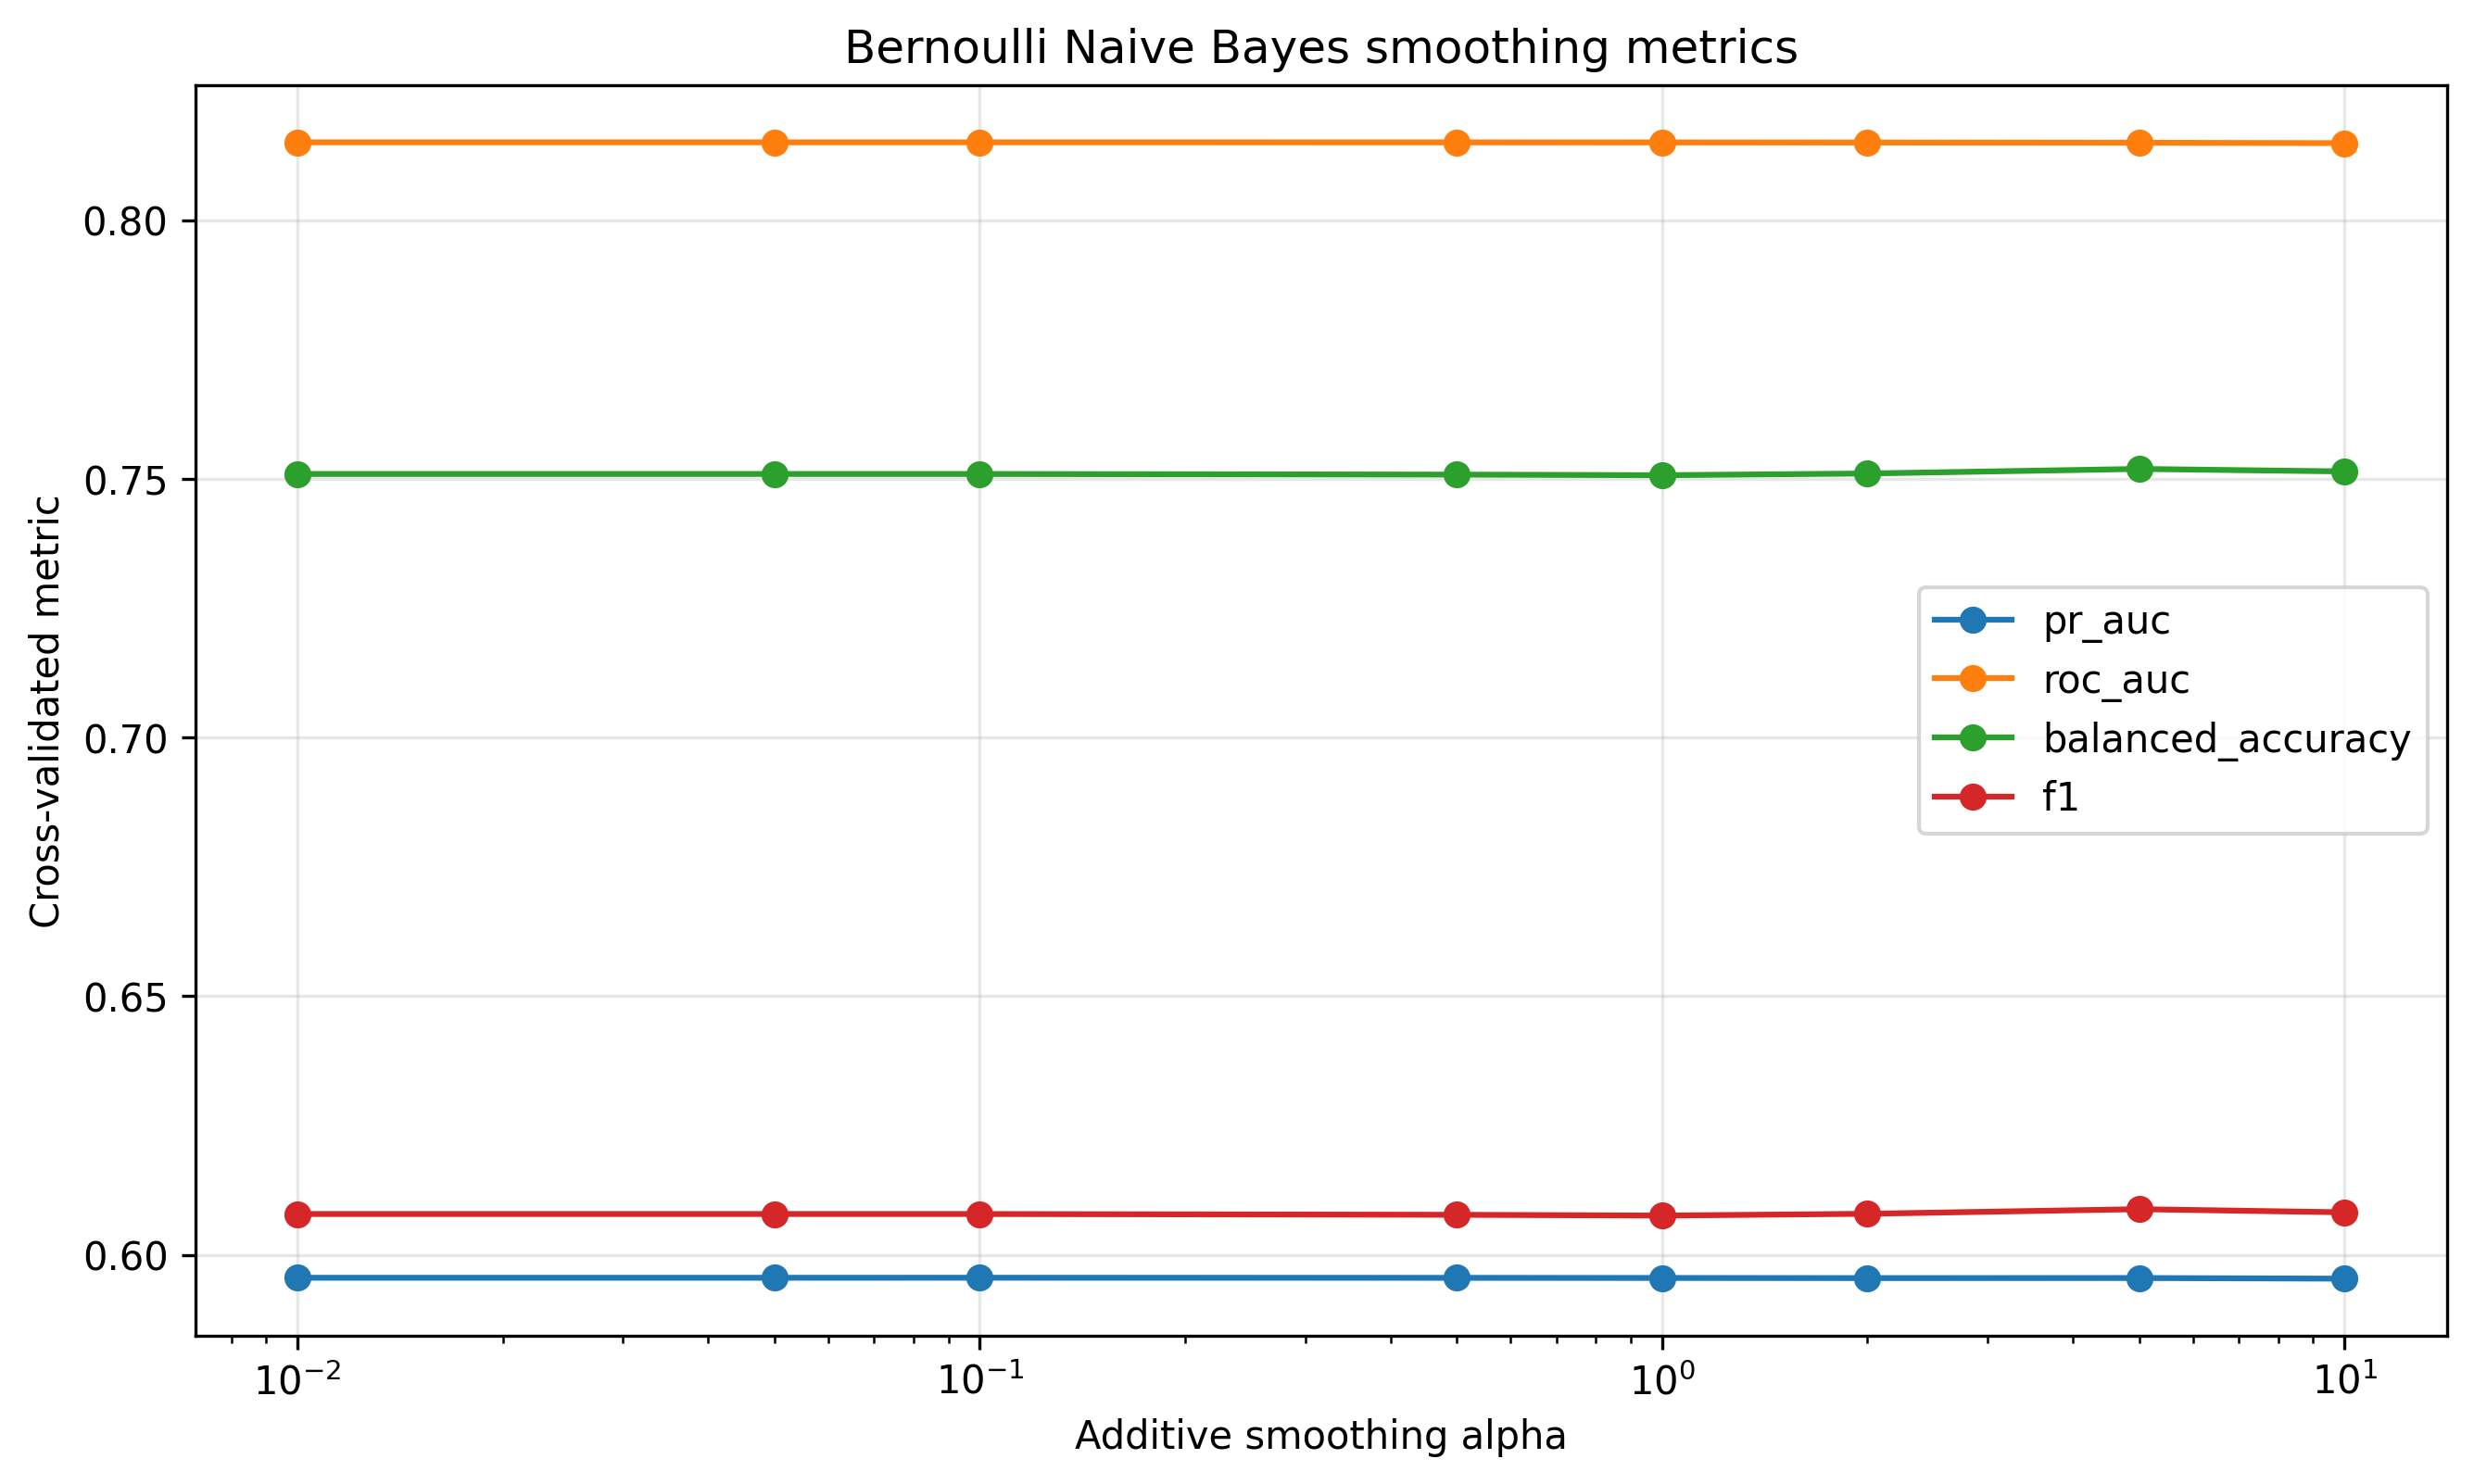
\includegraphics[width=0.82\textwidth]{../figures/bernoulli_nb_alpha_metrics.png}
\caption{Bernoulli Naive Bayes smoothing metrics}
\label{fig:bernoulli-nb-alpha}
\end{figure}

For example, PR-AUC remains around \(0.596\) across the grid, ROC-AUC remains around \(0.815\), and balanced accuracy remains close to \(0.751\). This stability suggests that the categorical indicator likelihoods are not overly sensitive to rare zero-probability problems under this cross-validation setup.

\subsection{Threshold behaviour}

Figure~\ref{fig:nb-threshold-tradeoff} shows the threshold tradeoff for the selected full transformed Gaussian Naive Bayes model. The curve is strikingly flat compared with the threshold curves for logistic regression and kNN. Even when the threshold increases from \(0.05\) to \(0.80\), recall remains high, while precision increases only gradually.

\begin{figure}[H]
\centering
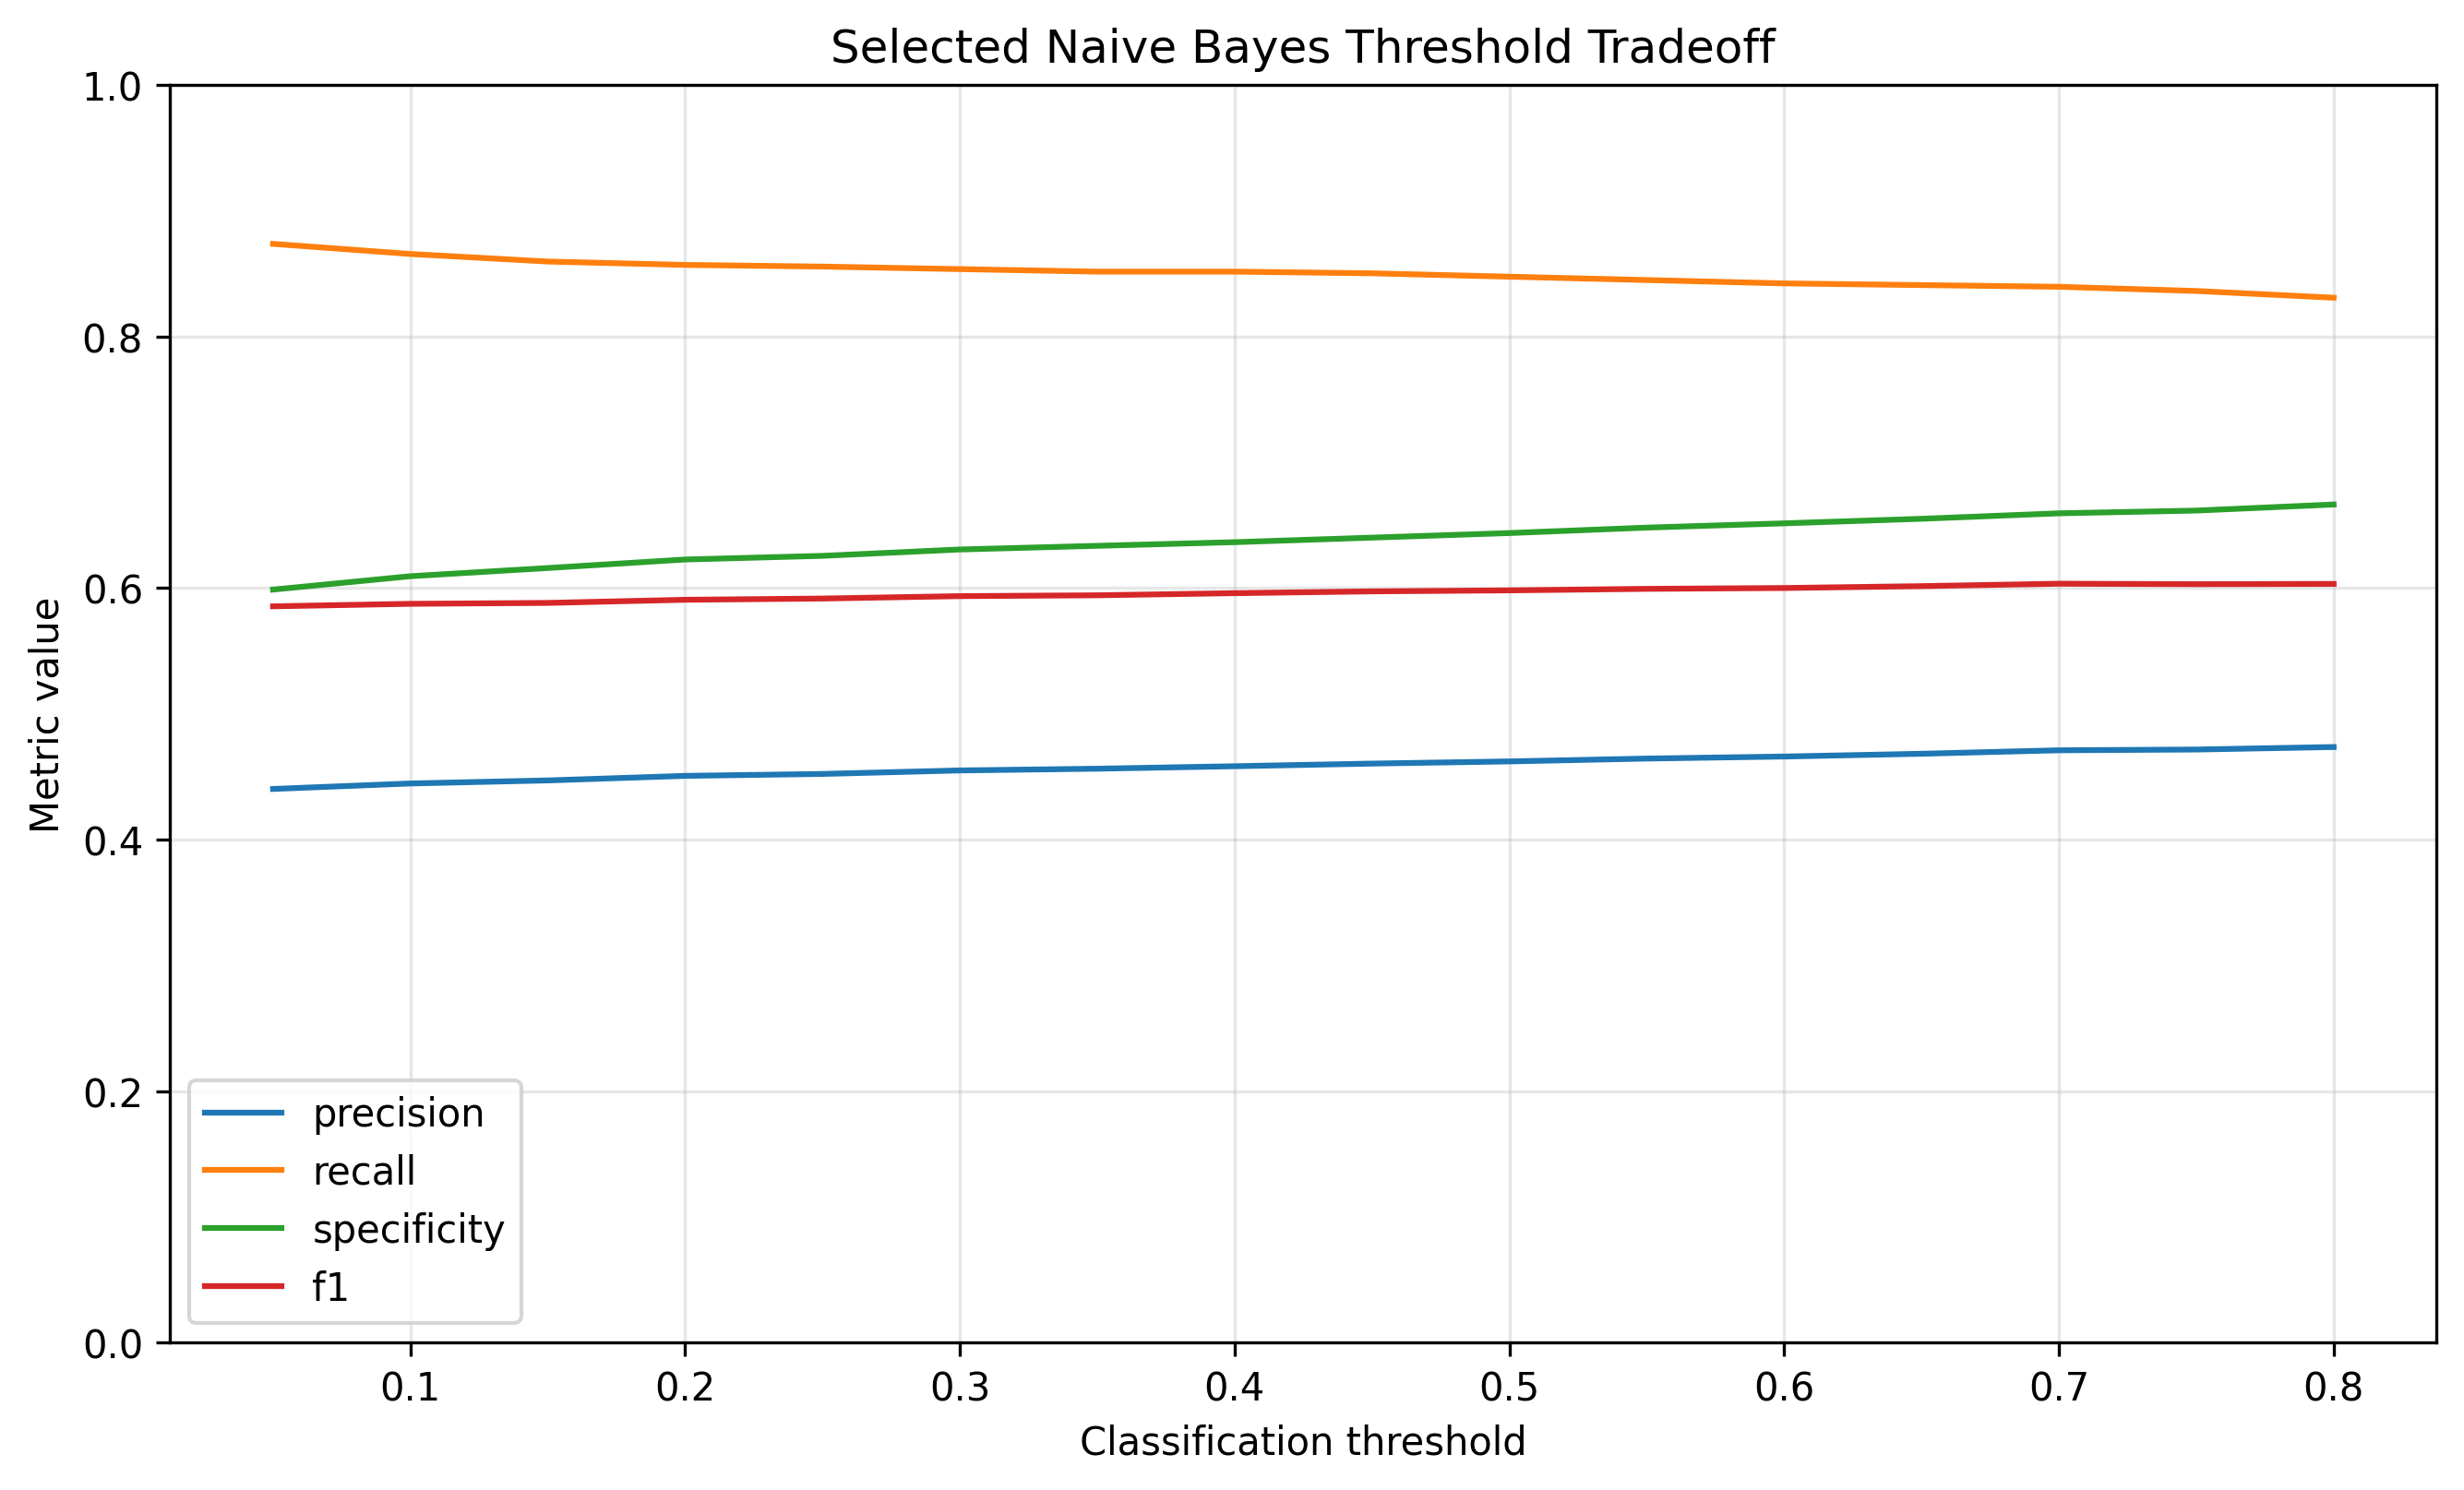
\includegraphics[width=0.88\textwidth]{../figures/naive_bayes_threshold_tradeoff.png}
\caption{Threshold tradeoff for the selected Naive Bayes model}
\label{fig:nb-threshold-tradeoff}
\end{figure}

At threshold \(0.50\), the selected model has precision approximately \(0.462\), recall approximately \(0.847\), specificity approximately \(0.644\), and \(F_1\) approximately \(0.598\). At threshold \(0.95\), recall is still approximately \(0.813\), while precision only rises to approximately \(0.492\). This indicates that many predicted probabilities are pushed toward high values. Such overconfident probabilities are consistent with the Naive Bayes independence assumption being violated by correlated feature groups.

This does not mean that the model is useless. It ranks customers much better than chance. However, it suggests that Naive Bayes probability levels should not be interpreted as calibrated churn probabilities without further calibration analysis.

\subsection{ROC and precision-recall curves}

Figure~\ref{fig:nb-roc-curve} shows the ROC curve for the selected Naive Bayes model. The ROC-AUC is approximately \(0.819\), clearly above the random-ranking line. This confirms that Naive Bayes learns meaningful churn-discriminating structure.

\begin{figure}[H]
\centering
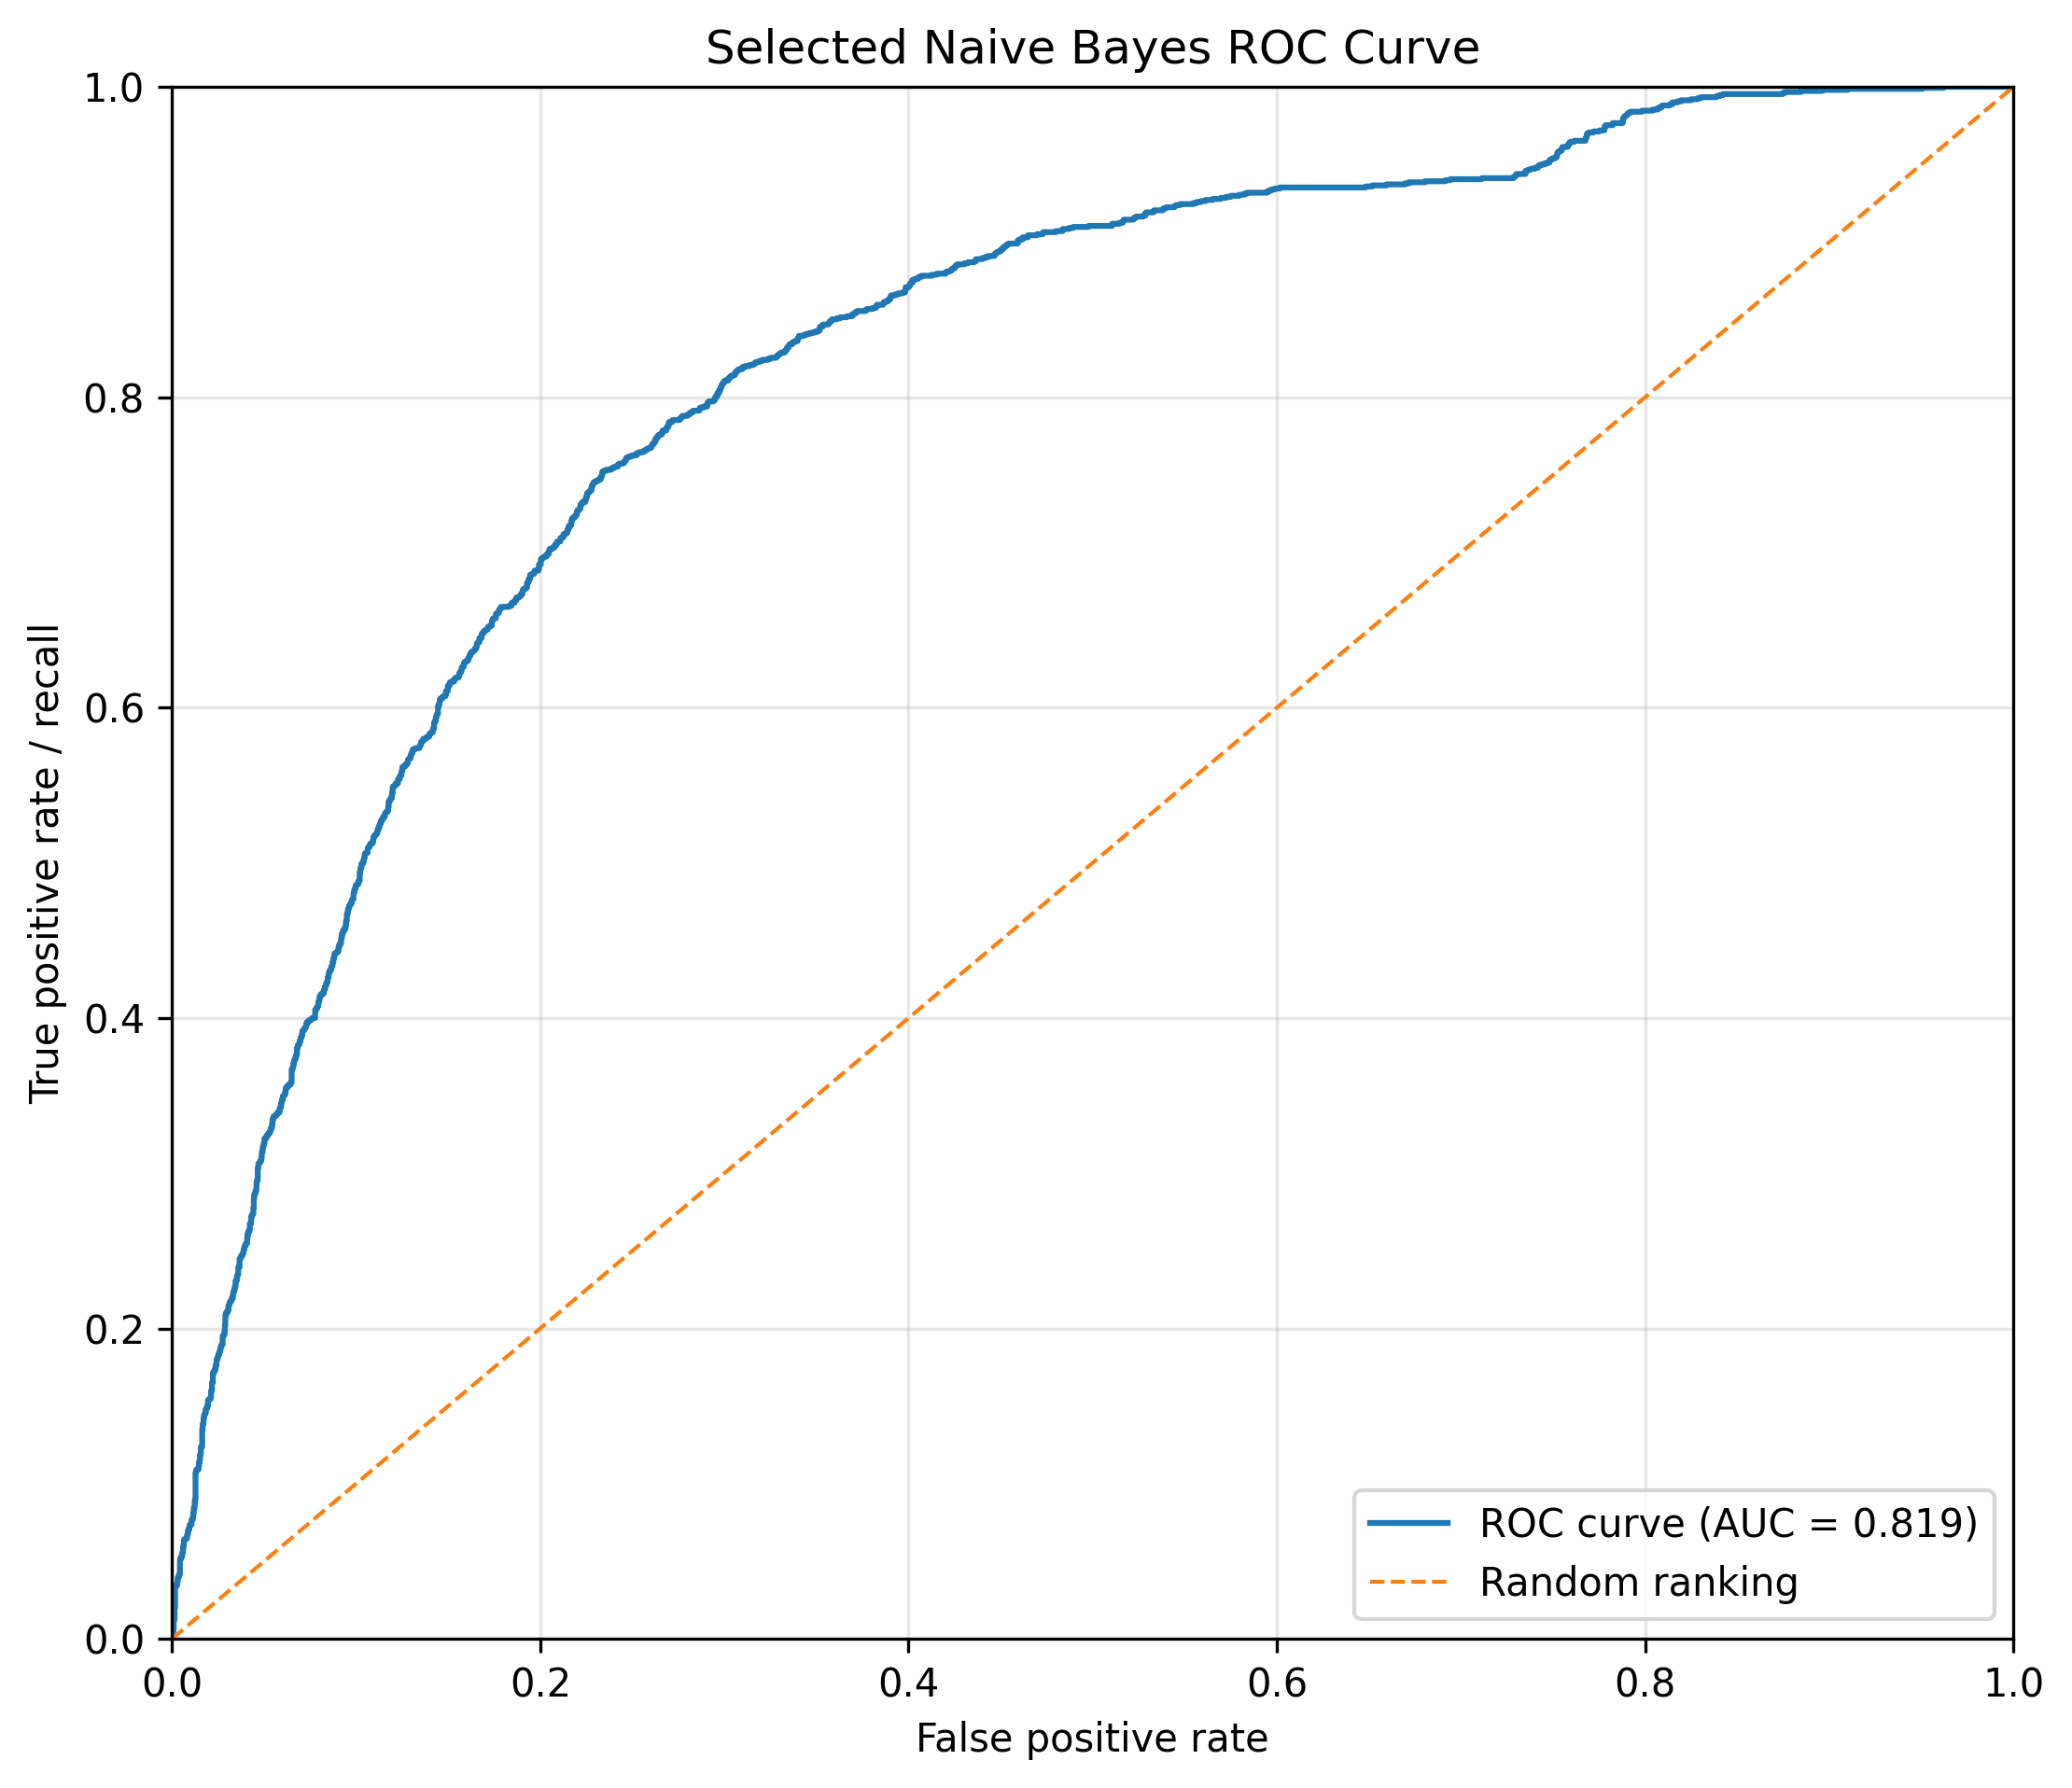
\includegraphics[width=0.72\textwidth]{../figures/naive_bayes_roc_curve.png}
\caption{ROC curve for the selected Naive Bayes model}
\label{fig:nb-roc-curve}
\end{figure}

Figure~\ref{fig:nb-pr-curve} shows the precision-recall curve. The PR-AUC is approximately \(0.604\), well above the positive-rate baseline of approximately \(0.265\). This indicates useful positive-class retrieval ability. However, the PR-AUC remains lower than the corresponding logistic regression and kNN values, so Naive Bayes is not the strongest ranking model so far.

\begin{figure}[H]
\centering
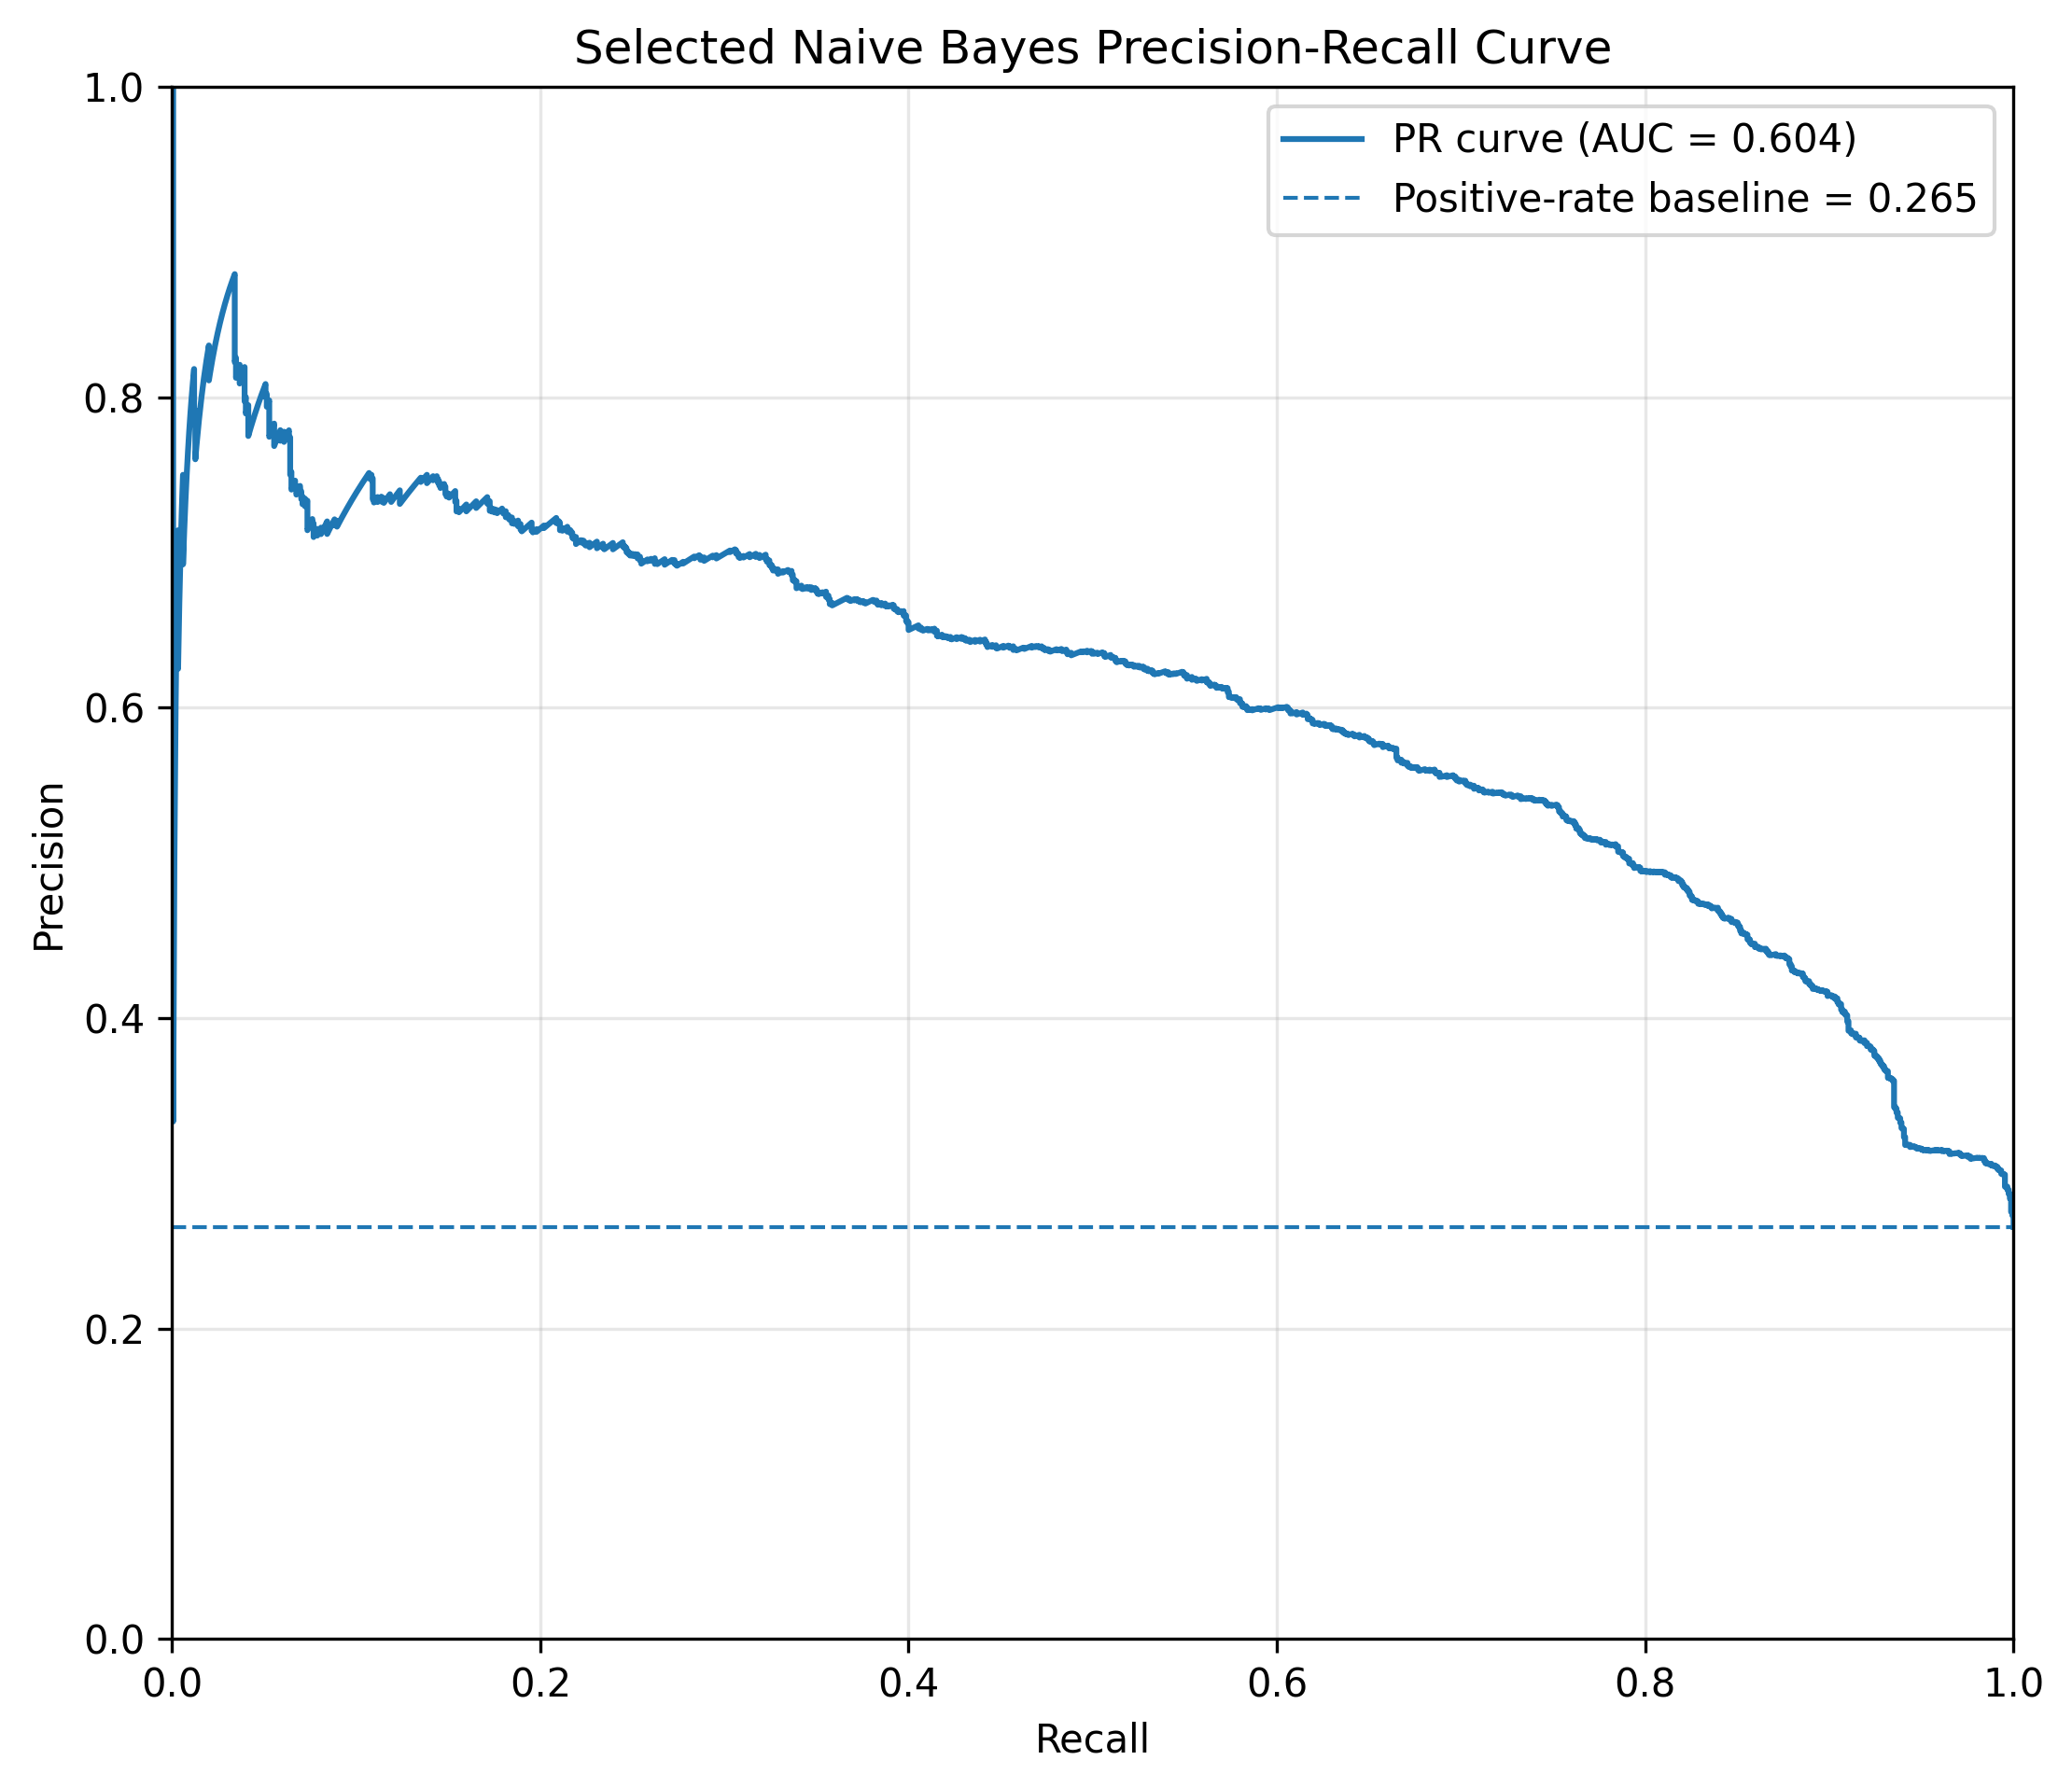
\includegraphics[width=0.72\textwidth]{../figures/naive_bayes_precision_recall_curve.png}
\caption{Precision-recall curve for the selected Naive Bayes model}
\label{fig:nb-pr-curve}
\end{figure}

\subsection{Summary}

The Naive Bayes experiment shows that a simple generative model can capture meaningful churn patterns. The selected full transformed Gaussian Naive Bayes model has high recall and useful ROC-AUC and PR-AUC. It is especially good at detecting many churners, but it does so by flagging a large fraction of the customer base.

The main limitation is probability behaviour. Because many Telco features are correlated, the conditional-independence assumption is not realistic. This likely causes related evidence to be counted multiple times and produces overconfident predicted probabilities. The threshold curve reflects this: increasing the threshold does not reduce recall as sharply as expected, and precision remains relatively low.

Compared with the learned models evaluated so far, Naive Bayes is useful but not dominant. Logistic regression remains the strongest model family so far by PR-AUC and ROC-AUC, while kNN is also stronger than Naive Bayes on these ranking metrics. Nevertheless, Naive Bayes adds an important modelling perspective: it connects classification to Bayes' rule, class priors, class-conditional likelihoods, smoothing, and the difference between ideal Bayes classification and practical approximate generative modelling.
